%!TEX root = ../prueba.tex
En este capítulo se pueden encontrar los requerimientos iniciales del sistema que se identificaron durante la toma de requerimientos y de una lluvia de ideas.

\section{Requerimientos Funcionales}
%!TEX root = ../prueba.tex
\begin{ReqSpec}
	\Req{REQMU01}{Iniciar Sesión}{Autenticación}{Funcional}{Como usuario de la aplicación requiero de un mecanismo que me permita escribir mi correo electrónico o nombre de usuario y una contraseña, con el fin de autenticar mi persona y así realizar acciones dentro de la aplicación web o móvil que correspondan a mi perfil. Las acciones que puedo realizar en el sistema deben ser desplegadas en un menú.}{Alta}
	
	\Req{REQMU02}{Crear, modificar y eliminar cuenta de usuario}{Autenticación}{Funcional}{Como cliente y proveedor del sistema requiero de un mecanismo que permita ingresar mis datos personales: nombres y apellidos, teléfono móvil, correo electrónico, escuela o unidad académica, comida preferida, nombre de usuario y contraseña para así tener una forma de autenticarme y acceder a las funcionalidades de la aplicación de acuerdo a mi perfil. También requiero de un mecanismo que me permita modificar mis datos personales de la cuenta o eliminar mi cuenta en caso de ya no requerirla.}{Alta}
	
	\Req{REQMU03}{Recuperar Cuenta de Usuario}{Autenticación}{Funcional}{Como usuario de la aplicación requiero de un mecanismo que me permita recuperar mis datos de acceso al sistema en caso de extraviar u olvidar mi cuenta de usuario o contraseña envíandome un correo electrónico o mensaje SMS los datos actualizados.}{Alta}

	\Req{REQMU04}{Vincular cuenta de Google}{Autenticación}{Funcional}{Debe existir un mecanismo que como usuario me permita vincular una cuenta existente del proveedor de servicio Google con el fin de identificarme dentro de la aplicación y tener acceso a los servicios que correspondan segun el rol.}{Baja}
	
	\Req{REQMU05}{Vincular cuenta de Facebook}{Autenticación}{Funcional}{Debe existir un mecanismo que como usuario me permita vincular una cuenta existente del proveedor de servicio  Facebook con el fin de identificarme dentro de la aplicación y tener acceso a los servicios que correspondan segun el rol.}{Baja}
	\Req{REQMU06}{Iniciar Sesión con una cuenta temporal}{Autenticación}{Funcional}{Debe existir un mecanismo}{Baja}
\end{ReqSpec}
%!TEX root = ../prueba.tex
\begin{ReqSpec}
	\Req{REQMP01}{Agregar Nuevo Establecimiento, Editar Información de Establecimiento y Eliminar Establecimiento}{Proveedor de Servicio}{Funcional}{Como proveedor del servicio de cafetería requiero de un mecanismo que me permita agregar la información de mi establecimiento: nombre, descripción, ubicación geográfica, escuelas más cercanas y especialidades, también se requiere de un mecanismo que me permita actualizar o editar la información previamente mencionada o eliminar la información de mi establecimiento para que ya no aparezca en la lista de establecimientos.}{Alta}
	
	\Req{REQMP02}{Agregar Información de Proveedor, Editar Información de Proveedor y Eliminar proveedor}{Proveedor de Servicio}{Funcional}{Como proveedor de servicio requiero de un mecanismo que me permita tener un control de las empresas a las que se les pide generalmente productos, los datos que se deberán registrar de los proveedores son: nombre de la empresa, lista de productos que surte, teléfono de contacto y correo electrónico. Así mismo requiero de un mecanismo que me permita actualizar los datos previamente enunciados y de un mecanismo que me permita eliminar la información de un proveedor.}{Baja}
	
	\Req{REQMP03}{Agregar Producto a Inventario, Editar Información del Producto y Eliminar Producto de Inventario}{Proveedor de Servicio}{Funcional}{Como proveedor del servicio requiero de un mecanismo que me permita agregar la siguiente información de nuevos productos adquiridos:nombre, descripción, clasificación del producto, imagen, precio de venta, precio de adquisición. Así mismo, requiero de un mecanismo que me permita actualizar la información de un producto de mi inventario o eliminarlo en caso de haber un registro erróneo en la aplicación.}{Alta}
	
	\Req{REQMP04}{Registrar entrada de productos a la cafetería}{Proveedor de Servicio}{Funcional}{Como proveedor del servicio requiero de un mecanismo que me permita indicar cuando un pedido hecho a un proveedor llega a la cafetería para que esos productos pasen a formar parte de lo que se puede vender en el día. La información que requiero que se registre es: nombre de la persona que recibe, hora de entrada de los productos, la lista de productos y la cantidad de los productos en unidades, estado general del pedido y el estado particular de los productos.}{Alta}
	
	\Req{REQMP09}{Actualizar existencia de producto}{Proveedor de Servicio}{Funcional}{Como proveedor de servicio requiero de un mecanismo que por cada producto que sea vendido se actualice su existencia dentro de la cafetería con el fin de tener un control de los productos que todavía pueden ser vendidos.}{Alta}
		%Cambia el estado 
			%Stock > 10
			%A punto de agotarse 0 < p < 10
			%Agotado = 0
			
	\Req{REQMP05}{Agregar paquete, Editar Paquete y Eliminar Paquete}{Proveedor de Servicio}{Funcional}{Como proveedor de servicio requiero de un mecanismo que me permita armar paquetes para que los clientes compren de 3 a 5 productos con una reducción del costo configurable de entre 5\% y 10\% sobre el costo total de los productos que conforman el producto además de poder darle un nombre, descripción e imagen. También requiero de un mecanismo que me permita actualizar los productos que conforman un paquete, su precio, nombre, descripción e imagen.}{Alta}
	%Paquete 1:
		%Cafe
		%Torta
		%Gelatina
		
	\Req{REQMP06}{Consultar lista de pedidos}{Proveedor de Servicio}{Funcional}{Como proveedor de servicio requiero de un mecanismo que me permita consultar los pedidos de un establecimiento que están confirmados y en espera para seleccionar aquellos pedidos voy a cocinar o que estoy a punto de acabar para que el cliente pase por el.}{Alta}
	
	\Req{REQMP07}{Consultar pedido}{Proveedor de Servicio}{Funcional}{Como proveedor de servicio requiero de un mecanismo que me permita seleccionar un pedido y consultar las especificaciones del cliente.}{Alta}
	
	
	\Req{REQMP08}{Actualizar estado del pedido}{Proveedor de Servicio}{Funcional}{Como proveedor de servicio requiero de un mecanismo que:
		\begin{Citemize}
			\item Permita al cliente indicar que confirma su pedido, que cancela su pedido, que ha ido ha la caja y pagado su pedido.
			\item Me permita indicar que estoy preparando un pedido o que estoy a punto de terminar su preparación o me permita indicar cuando un pedido puede ser recogido por otro cliente cuando el que lo solicitó tardo más de 10 minutos en recogerlo.
		\end{Citemize}}{Alta}
		%Actualizar
			%Por confirmar
			%En espera
			%En preparación
			%A punto de terminar
			%Recogido y pagado
			%Cancelado
			%En espera de nuevo cliente
			
	\Req{REQMP10}{Reporte de la Experiencia del Cliente}{Proveedor de Servicio}{Funcional}{Como proveedor de servicio requiero de un mecanismo que me permita consultar la experiencia promedio de los clientes que visitan el establecimiento.}{Baja}
	
	\Req{REQMP11}{Agregar promoción, editar promoción, guardar promoción y eliminar promoción}{Proveedor de Servicio}{Funcional}{Como proveedor de servicio requiero de un mecanismo que me permita registrar promociones en la aplicación con los siguientes datos: nombre, periodo de vigencia, productos que entran en la promoción y criterios que los clientes deben cumplir para entrar en la promoción. Así mismo requiero de un mecanismo que me permita modificar los datos previamente descritos. También se requiere de un mecanismo que me permita almacenar los datos relacionados a una promoción para posteriormente volver a utilizarla, así como también un mecanismo que me permita eliminar los datos referentes a una promoción siempre y cuando no haya ventas ya realizadas con la promoción.}{Media}
	
	\Req{REQMP12}{Reporte promedio de Entradas/Salidas}{Proveedor de Servicio}{Funcional}{Como proveedor de servicio requiero de un mecanismo que me permita conocer cuantos productos entran a la cafetería por medio de proveedores y cuantos salen por pedidos o ventas en caja. El rango del tiempo de este mecanismo debe ser de un mes a un año.}{Baja}
	
	\Req{REQMP13}{Reporte de productos más consumidos}{Proveedor de Servicio}{Funcional}{Como proveedor de servicio requiero de un mecanismo que me permite conocer cuales son los productos que más se venden.}{Baja}
	
	\Req{REQMP15}{Venta en Caja}{Proveedor de Servicio}{Funcional}{Como proveedor de servicio requiero de un mecanismo que me permita surtir pedidos de clientes que vienen directamente al establecimiento.}{Alta}
\end{ReqSpec}

%!TEX root = ../prueba.tex
\begin{ReqSpec}
	\Req{REQMPD01}
	{Programar Pedido}
	{Pedidos}
	{Funcional}
	{Como cliente requiero de un mecanismo para programar un pedido, es decir, solicitar al servicio de cafeteria que realice un pedido en el tiempo que yo lo solicite.}
	{Alta}
	
	\Req{REQMPD02}{Realizar Pedido}{Pedidos}{Funcional}{Como cliente requiero de un mecanismo que me permita efectuar un pedido una vez que haya elegido los pruductos que quiero solicitar.}{Alta}
	\Req{REQMPD03}{Agregar producto a pedido}{Pedidos}{Funcional}{Como cliente requiero una herramienta de sistema que me permita agregar más de un producto a la lista de productos de mi pedido y así realizar un solo pago o realizar una vez el pedidio sin necesidad de hacerlo cada vez que quiera un producto.}{Alta}
	\Req{REQMPD04}{Calificar el servicio}{Pedidos}{Funcional}{Como cliente requiero una herramienta del sistema que me permita calificar el servicio de cafetería en el cual realicé una compra de algún producto y con base en la calificación que se otorgue, otros usuarios con base en su criterio se percaten del tipo de servicio que otorga la cafeteria.}{Baja}
	%\Req{REQMPD05}{Actualizar estado del pedido}{Pedidos}{Funcional}{Como proveedor requiero una herramienta de sistema que me permita realizar la actualización de los productos, es decir modificar el estado en el que se encuentra el pedido solicitado y así notificar al usuario cualquier cosa referente al pedido realizado.}{Alta}
	\Req{REQMPD06}{Encontrar establecimientos por un filtro}{Pedidos}{Funcional}{Como cliente requiero una herramienta del sistema que me permita encontrar los distintos establecimientos en los que puedo adquirir los productos.}{Media}
	\Req{REQMPD07}{Consultar lista de productos del cliente}{Pedidos}{Funcional}{Como cliente requiero una herramienta de sistema que me permita visualizar los productos que voy a encargar al servicio de cafeteria y así asegurarme de los productos que estoy solicitando y el dinero que voy a requerir para solicitarlos.}{Media}
\end{ReqSpec}
%!TEX root = ../prueba.tex
\begin{ReqSpec}
	
	\Req{REQMPG01}
	{Pagar en caja con efectivo}
	{Pagos}
	{Funcional}
	{Como proveedor del servicio requiero de un mecanismo para recibir pagos en caja por mis productos y/o servicios en efectivo, así mismo como cliente requiero de un mecanismo para efectuar pagos  en caja por compras en efectivo.}
	{Alta}
	
	\Req{REQMPG02}
	{Pagar en caja con tarjeta de crédito/débito}
	{Pagos}
	{Funcional}
	{Como proveedor del servicio requiero tener un mecanismo para recibir pagos por tarjeta de crédito/débito en caja por mis productos y/o servicios, así mismo como cliente requiero de un mecanismo para efectuar pagos en caja por compras con tarjeta de crédito/débito.}
	{Media}
	
	\Req{REQMPG03}
	{Pagar con una cuenta en PayPal}
	{Pagos}
	{Funcional}
	{Como proveedor del servicio requiero tener un mecanismo para recibir pagos por PayPal por mis productos y/o servicios, así mismo como cliente requiero de un mecanismo para efectuar pagos por compras con PayPal.}
	{Alta}
	
	\Req{REQMPG04}
	{Pagar con una tarjeta de crédito/débito}
	{Pagos}
	{Funcional}
	{Como proveedor del servicio requiero tener un mecanismo para recibir pagos por tarjeta de crédito/débito por mis productos y/o servicios realizados por medio de la plataforma de la aplicación, así mismo como cliente requiero de un mecanismo para efectuar pagos por compras con tarjeta de crédito/débito por medio de la plataforma de la aplicación.}
	{Media}
	
	\Req{REQMPG05}
	{Agregar tarjeta de crédito/débito}
	{Pagos}
	{Funcional}
	{Como cliente requiero de un mecanismo para poder agregar mi tarjeta de crédito/débito a mi cuenta para poder efectuar pagos por los productos y/o servicios adquiridos.}
	{Media}	

\end{ReqSpec}

\section{Requerimientos No Funcionales}
%!TEX root = ../prueba.tex
\begin{ReqSpec}
	\Req{REQNF01}{Integridad Lógica de Datos}{No Aplica}{No Funcional}{La aplicación móvil proveerá al Cliente únicamente la información de cafeterías, locales y productos que hayan sido publicados en el sistema.}{Media}
	\Req{REQNF02}{Extensibilidad}{No Aplica}{No Funcional}{Se hará huso de la descripción de tipo de Caja Negra proveyendo de los elementos con mayor relevancia para el negocio.}{Alta}
	\Req{REQNF03}{Tolerancia a Fallos}{No Aplica}{No Funcional}{}{Media}
	\Req{REQNF04}{Integrabilidad}{No Aplica}{No Funcional}{}{Media}
\end{ReqSpec}

\section{Casos de Uso}
Una ves que se han presentado los requerimientos funcionales del sistema, utilizamos un diagrama de casos de uso que servirá para definir el alcance del proyecto al finalizar el periodo escolar 2018-2019/1. Este diagrama de casos de uso se puede observar en la figura \ref{fig:casosDeUso}.

\begin{figure}[hbtp!]
	\begin{center}
		\fbox{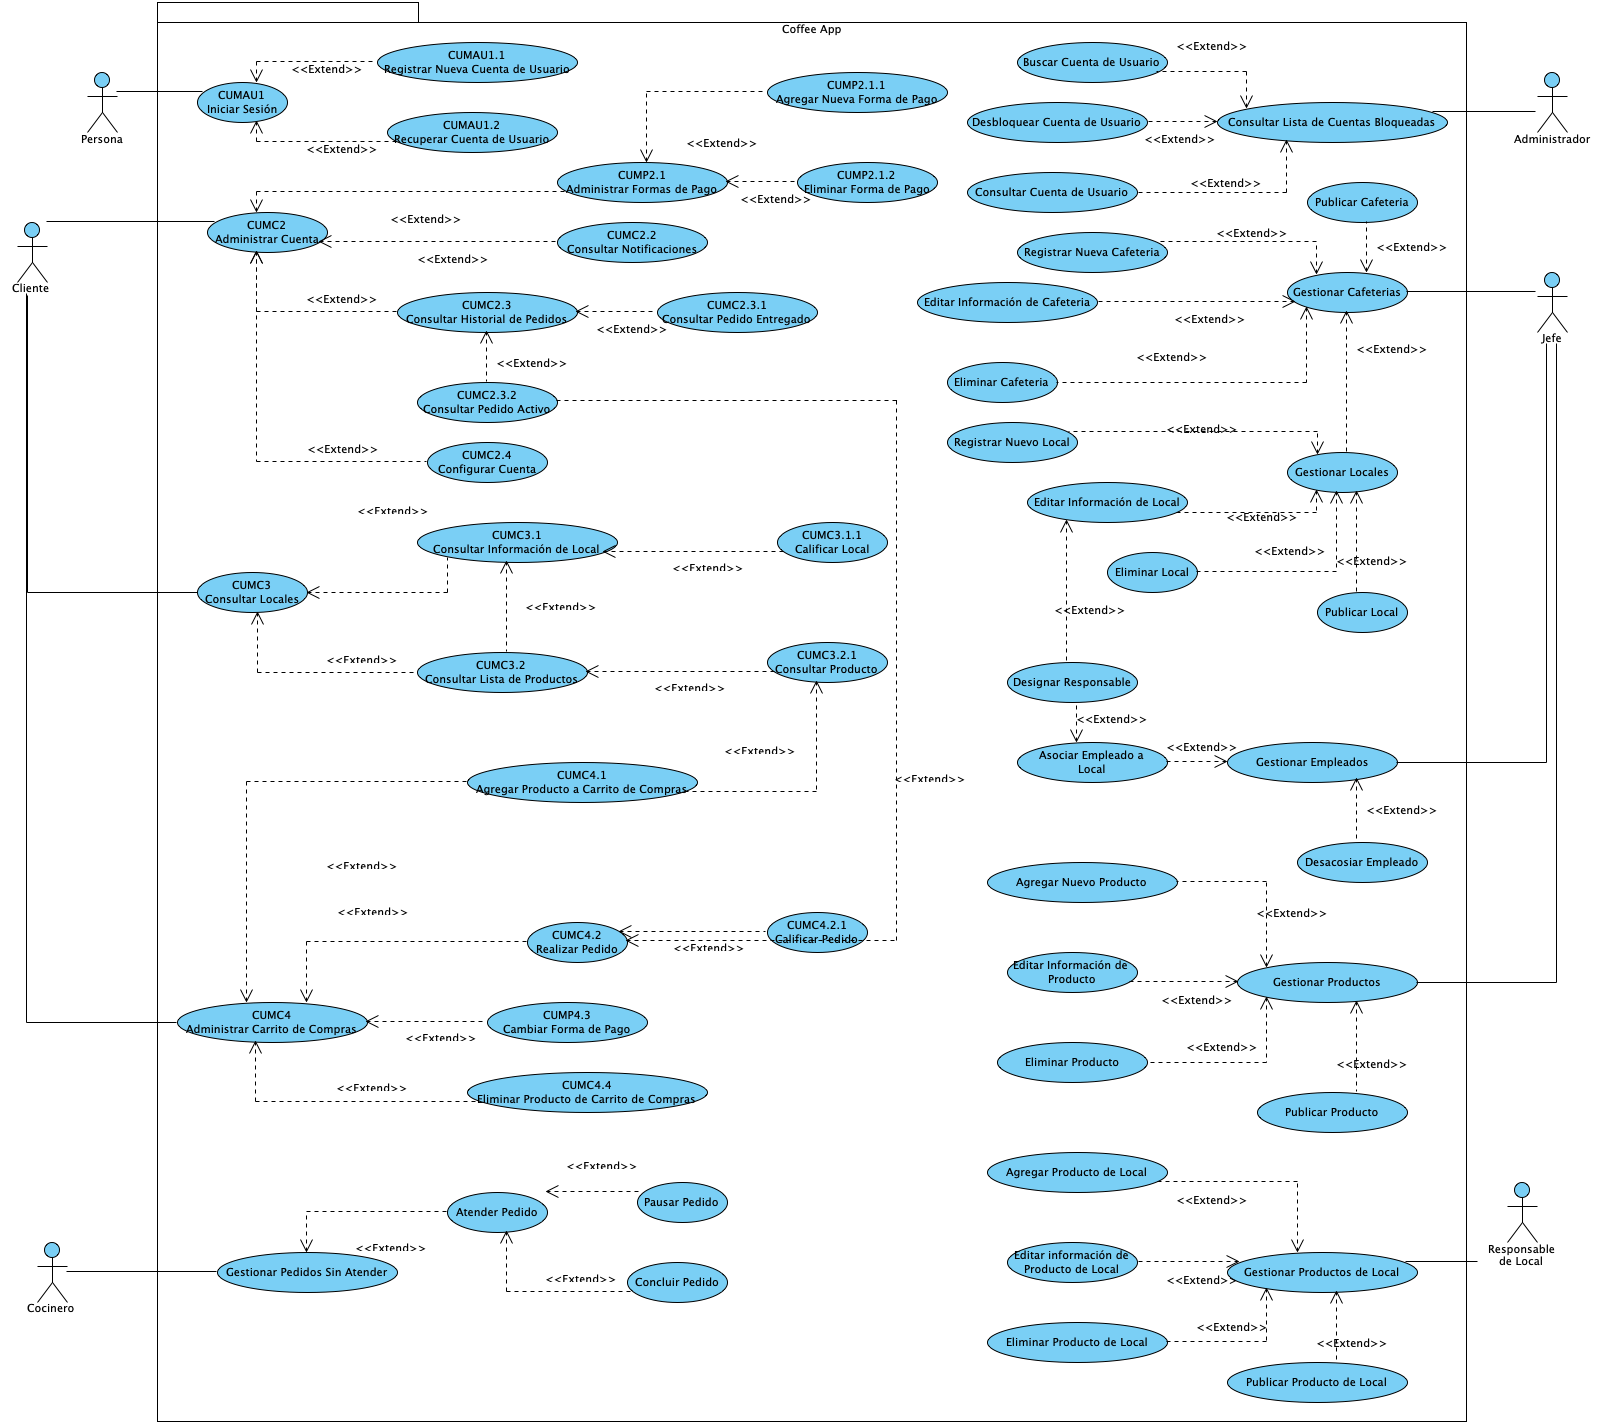
\includegraphics[angle=90,width=\textwidth]{img/cus}}
		\caption{Diagrama de Casos de Uso}
		\label{fig:casosDeUso}
	\end{center}
\end{figure}


\section{Interfaces de Usuario}
En la figura \ref{fig:mapaDeNavegacion} se utiliza una máquina de estados para presentar el camino ideal que se debe seguir para el uso de la aplicación móvil.

\begin{figure}[hbtp!]
	\begin{center}
		\fbox{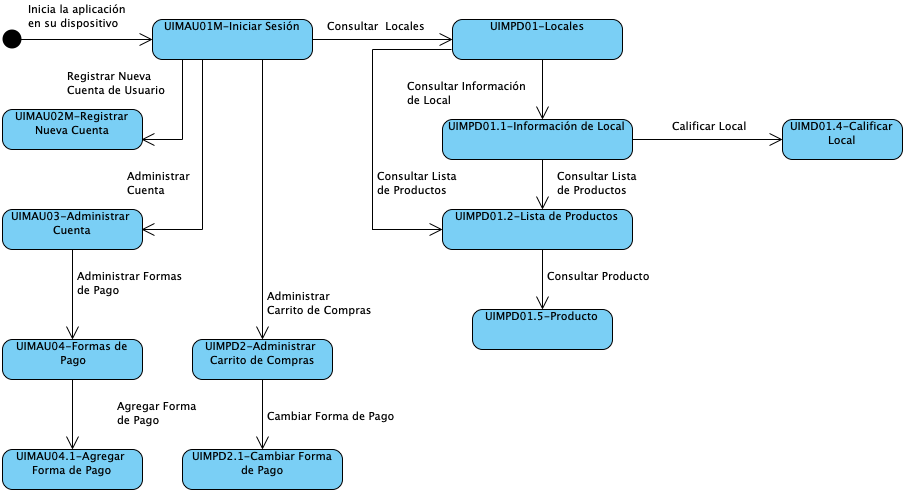
\includegraphics[width=0.8\textwidth]{img/mapaDeNavegacion}}
		\caption{Mapa de Navegación}
		\label{fig:mapaDeNavegacion}
	\end{center}
\end{figure}

%%!TEX root = ../../prueba.tex
\begin{IU}{IUMC3}{Consultar Locales}{En esta pantalla se muestran los locales que están cerca de la ubicación del \getElementById[Stakeholder]{Cliente}. Así mismo el cliente podrá realizar la búsqueda de un Local sí conociese su nombre o algunas palabras de su nombre. La pantalla desplegará la siguiente información del local:	\begin{Citemize}
		\item \getElementById[Entidad]{local.foto}.
		\item \getElementById[Entidad]{local.nombreLocal}.
		\item \getElementById[Entidad]{local.horaInicio}.
		\item \getElementById[Entidad]{local.horaFin}.
	\end{Citemize}}{casosDeUso/cumc3/IUMC3}
	\item[Acciones]:\hspace{1pt}
		\begin{Citemize}
			\item Al seleccionar un local se mostrarán los productos que se ofertan en ese local tal como se describe en el caso de uso \getElementById[CU]{CUMC3.2}.
			\item Al ingresar texto \fbox{Buscar cafetería} se realizará la búsqueda de los locales que contengan parte del texto ingresado.
		\end{Citemize}

\end{IU}


